\section{GeSS}
{{\footnotesize
\begin{description}[labelwidth=5em, labelsep=1em, leftmargin=*, align=left, itemsep=0.3em, parsep=0em]
  \item[date:] 2024-12-13
  \item[last\_updated:] 2024-12
  \item[expired:] unkown
  \item[valid:] yes
  \item[url:] \href{https://neurips.cc/virtual/2024/poster/97816}{https://neurips.cc/virtual/2024/poster/97816}
  \item[domain:] Scientific ML; Geometric Deep Learning
  \item[focus:] Benchmark suite evaluating geometric deep learning models under real-world distribution shifts
  \item[keywords:]
    - geometric deep learning
    - distribution shift
    - OOD robustness
    - scientific applications
  \item[task\_types:]
    - Classification
    - Regression
  \item[ai\_capability\_measured:]
    - OOD performance in scientific settings
  \item[metrics:]
    - Accuracy
    - RMSE
    - OOD robustness delta
  \item[models:]
    - GCN
    - EGNN
    - DimeNet++
  \item[ml\_motif:]
    - Geometric DL
  \item[type:] Benchmark
  \item[ml\_task:] Classification, Regression
  \item[notes:] Includes no-OOD, unlabeled-OOD, and few-label scenarios :contentReference[oaicite:6]\{index=6\}.
  \item[contact.name:] Deyu Zou
  \item[contact.email:] unkown
  \item[results.name:] ChatGPT LLM
  \item[results.url:] \href{unkown}{unkown}
  \item[fair.reproducible:] Yes
  \item[fair.benchmark\_ready:] Yes
  \item[ratings.software.rating:] 0
  \item[ratings.software.reason:] Not analyzed.
  \item[ratings.specification.rating:] 9.0
  \item[ratings.specification.reason:] Well-defined problem (Tc prediction, generation) with strong scientific motivation (high-Tc materials), but no formal hardware constraints.
  \item[ratings.dataset.rating:] 9.0
  \item[ratings.dataset.reason:] Includes curated 3D crystal structures and Tc data; readily downloadable and used in paper models.
  \item[ratings.metrics.rating:] 9.0
  \item[ratings.metrics.reason:] MAE and structural validity used, well-established in materials modeling.
  \item[ratings.reference\_solution.rating:] 8.0
  \item[ratings.reference\_solution.reason:] Provides two reference models (SODNet, DiffCSP-SC) with results. Code likely available post-conference.
  \item[ratings.documentation.rating:] 8.0
  \item[ratings.documentation.reason:] Paper and poster explain design choices well; software availability confirms reproducibility but limited external documentation.
  \item[id:] gess
  \item[Citations:] \cite{neurips2024_a8063075}
  \item[Ratings:]
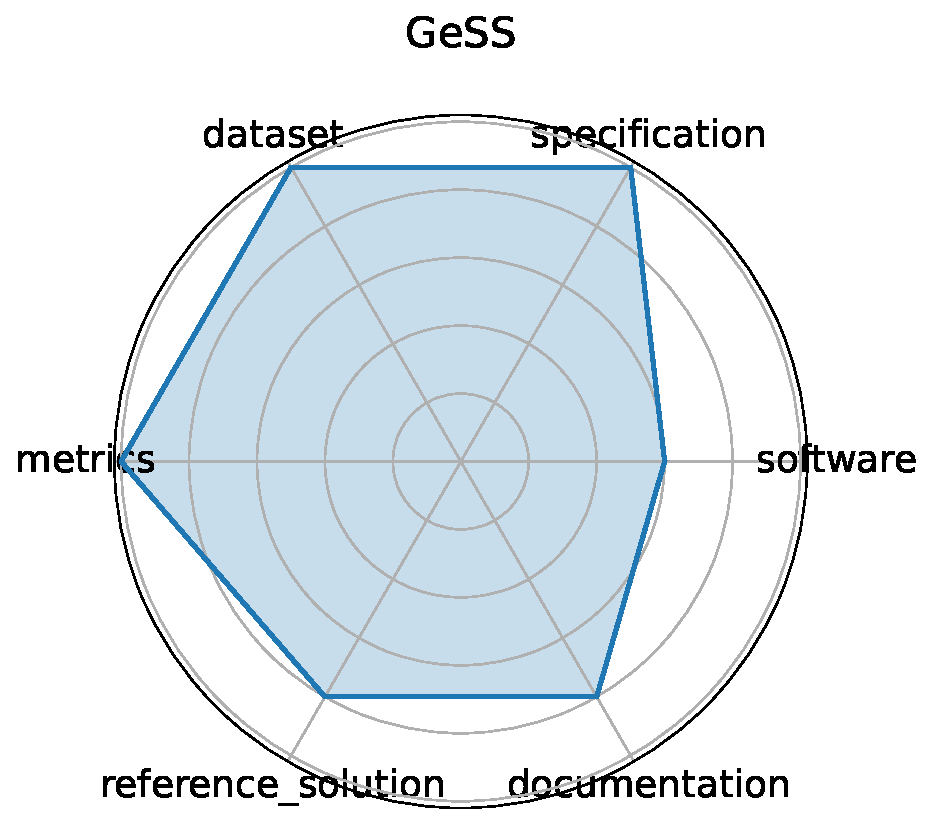
\includegraphics[width=0.2\textwidth]{gess_radar.pdf}
\end{description}
}}
\clearpage